\documentclass[11pt]{article}
\usepackage[utf8]{inputenc}
\usepackage[margin=1in]{geometry}
\usepackage{natbib}
\bibliographystyle{abbrvnat}
\usepackage{amsmath}
\usepackage{amssymb}
\usepackage{comment}
\usepackage{bbm}
\usepackage{amsthm}
\geometry{a4paper}
\usepackage{graphicx}
\usepackage{booktabs}
\usepackage{array}
\usepackage{paralist}
\usepackage{verbatim}
\usepackage{subfig}
\usepackage{multirow}
\usepackage{rotating}
\usepackage{fancyhdr}
\usepackage{hyperref}
\usepackage{bm}
\usepackage{xcolor}
\usepackage{listings}
\lstset{basicstyle=\ttfamily,
  showstringspaces=false,
  commentstyle=\color{red},
  keywordstyle=\color{blue}
}
\pagestyle{fancy}
\renewcommand{\headrulewidth}{0pt}
\lhead{}\chead{}\rhead{}
\lfoot{}\cfoot{\thepage}\rfoot{}
\usepackage{algorithm}
\usepackage{algpseudocode}
\usepackage{fancyvrb}
\usepackage{pythonhighlight}

\title{%
  Data Science - Coursework 2 \\
  \large Comparison of two methods for calculating \\ SHAP values for categorical variables.}
\date{May 2024}
\author{02344391}


\begin{document}

\maketitle
\section*{Introduction}
It is often necessary to explain the predictions made by a machine learning model in order to 
understand the model's decisions. The simplest models, such as linear regression models, can 
be explained by their coefficients. On the other hand, more complex models sometimes require 
the use of an explanatory model to locally explain the predictions associated with each input.

The \href{https://github.com/shap/shap}{SHAP} \textit{Python} module uses Shapley values from 
game theory to explain the predictions of a wide range of models.
According to \cite{lundberg2019consistent}, the module calculates the contribution $\phi_i$ for each 
feature $i$ given an input $u$ on a model $f$ by:

\begin{equation}
    \phi_i = \sum_{S \subseteq N \backslash \{i\}}\frac{|S|!(M-|S| - 1)!}{M !}[f_u(S\cup \{i\})-f_u(S)]
    \label{eq:shap}
\end{equation}

where $N$ is the feature set, $M = |N|$ and:
$$f_u(S) = \mathbb{E}[f(u)|u_S]$$
is the expected value of the function given a subset $S$ of the features of $u$.

In the case of tree-based or ensemble models such as random forest, the \texttt{TreeExpalainer}
class of \href{https://github.com/shap/shap}{SHAP} calculates the Shapley values of each feature 
in an input from the fitted trees. The algorithm calculates $f_u(S)$ in (\ref{eq:shap}) by 
traversing the branches of the decision tree according to the feature values of $S$. When a 
node of the tree corresponds to a feature not included in $S$, the algorithm descends both 
branches under this node. Each of these descents leads to a value. The contribution of the subgroup
$S$ is then the weighted sum of the values obtained by traversing the tree. The weighting corresponds 
to the proportion of samples that passed through the branches of the tree during training.

So we have a method to calculate the contribution of each variable in this kind of models. In this report, 
we will not investigate the consistency of this method for explaining predictions, 
but we will study the particular case where a model has categorical variables that have been 
encoded by One-Hot Encoding. In this case, Shapley values are associated with each of the encoded 
variables. One method to calculate the contribution of categorical variables as a whole is to sum 
the Shapley values of the encoded variables corresponding to the categorical variable. This method for 
calculating the Shapley values of a decision tree assumes that the sub-variables produced by encoding a 
categorical variable are independent. This assumption is inherently false: the encoded sub-variables should 
be considered as a whole when calculating the Shap values using the fitted trees.

The goal of this project is to modify the algorithm calculating the SHAP values of \\ \texttt{TreeExplainer} to consider 
the entire set of sub-variables of a categorical variable as known when it is part of $S$. Moreover, this project 
heavily relies on functions from \href{https://scikit-learn.org/stable/}{Scikit-learn} (\cite{scikit-learn}), some of which are modified 
(e.g. \texttt{sklearn.tree.plot\_tree}) or not, for visualizations, dataset construction, or machine learning model construction.
this project 

\section*{A simple example of a regression tree}

We illustrate the calculation of SHAP values for a short regression tree with a dataset containing a 
numerical variable $x$ and a categorical variable that has been encoded with one-hot encoding $\text{cat}_1$ and $\text{cat}_2$.
We plot in figure (\ref{fig:tree0}) the fitted tree. For the following, we want to analyse the prediction of the input 
$u = (u_x, u_{\text{cat}_1}, u_{\text{cat}_2}) = (60,0,1)$.

\begin{figure}[H]
    \centering
    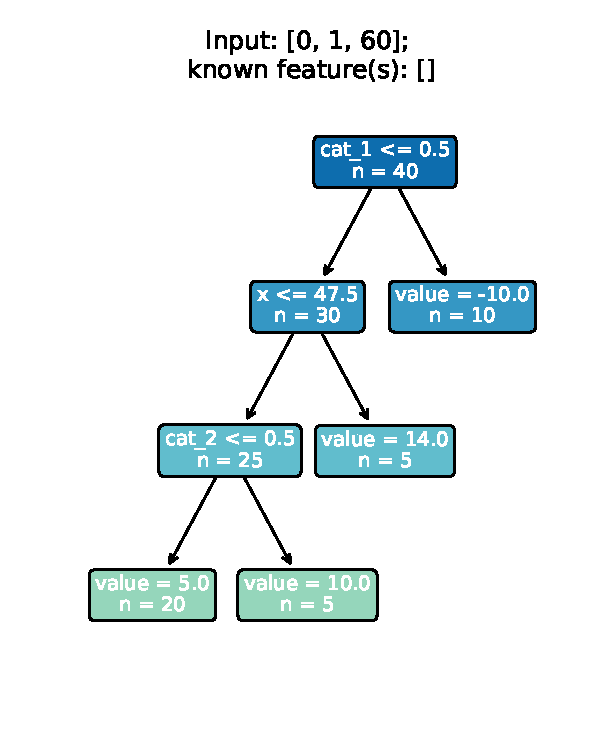
\includegraphics[height=9cm]{"../outputs/plot_tree/figures/path_0_known.pdf"}
    \caption{Plot of the fitted tree. The colored nodes correspond to the paths taken 
    by the algorithm when certain features of an input are known. Here, we consider that 
    no feature is known.}
    \label{fig:tree0}
\end{figure}

In figure (\ref{fig:tree0}), we consider that no feature is known, which corresponds to 
$$f_u(S) = f_u(\{\}) = \mathbb{E}[f(X)] = \frac{1}{40}\left(20 \times 5 + 5 \times 10 + 5 \times 14 + 10 \times (-10)\right)$$

the mean value of the prediction on the training set.

In figure (\ref{fig:tree1}), we plot the tree paths when one feature is known: $S = \{x\}$ or $S = \{\text{cat}_1 \}$ or $S = \{\text{cat}_2 \}$.
We find that 
\begin{align*}
    & f_u(\{\text{cat}_1 \}) = \frac{22}{3}\\
    & f_u(\{\text{cat}_2 \}) = \frac{11}{2}\\
    & f_u(\{ x \}) = 8
\end{align*}

\begin{figure}[H]
    \centering
    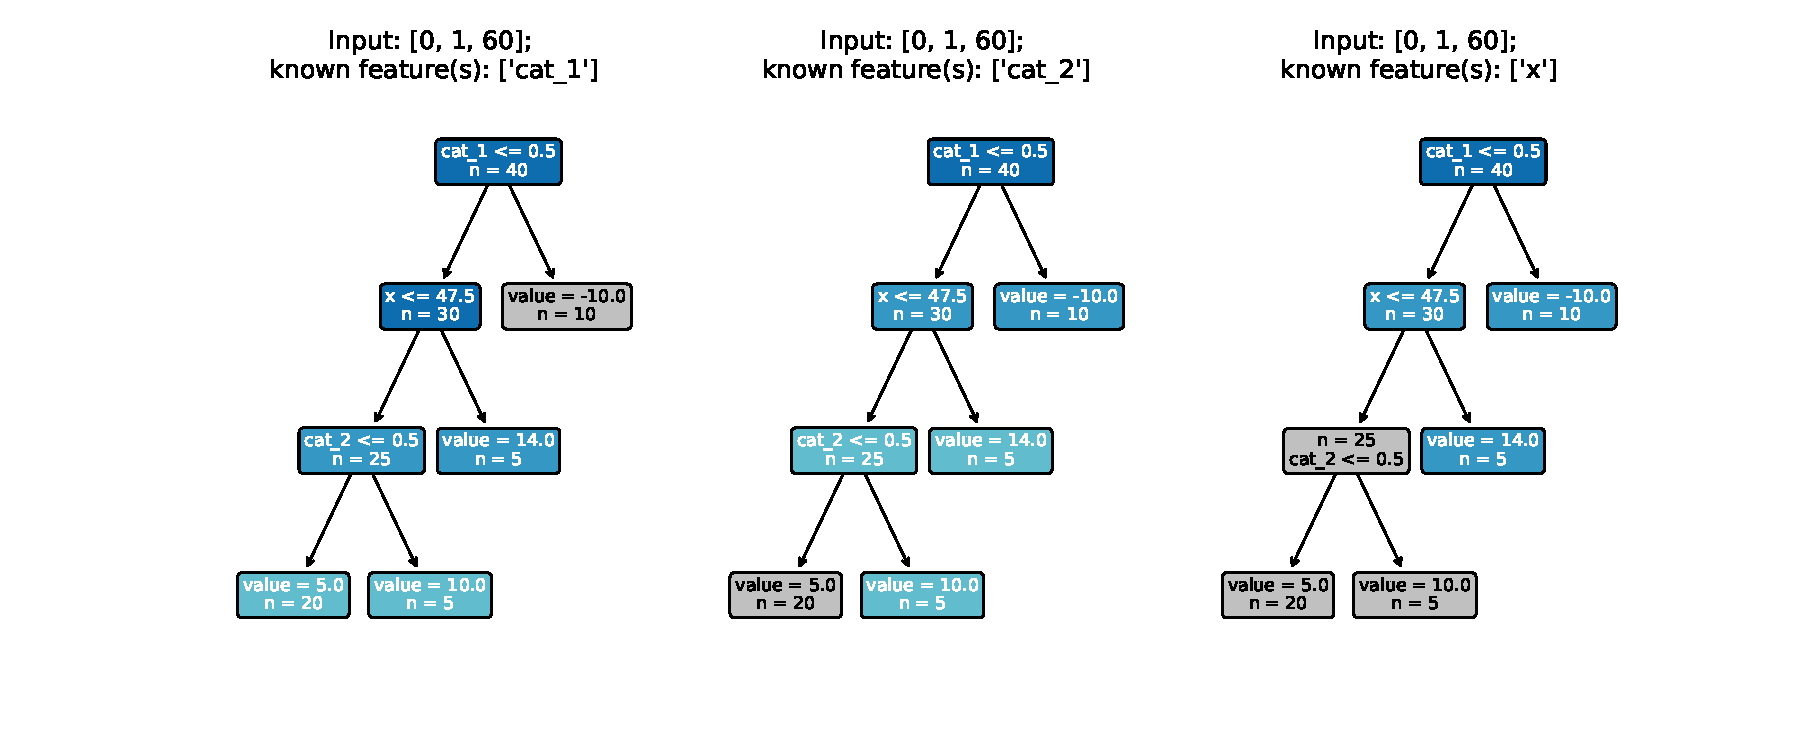
\includegraphics[height=6.6cm]{"../outputs/plot_tree/figures/path_1_known.pdf"}
    \caption{Plot of the fitted tree. The colored nodes correspond to the paths taken 
    by the algorithm when certain features of an input are known. Here, we consider that 
    one feature is known.}
    \label{fig:tree1}
\end{figure}

In figure (\ref{fig:tree2}), we plot the tree paths when two features are known: $S = \{\text{cat}_1, \text{cat}_2\}$ or $S = \{\text{cat}_2, x \}$ or $S = \{\text{cat}_1, x \}$.
We find that 
\begin{align*}
    & f_u(\{\text{cat}_1, \text{cat}_2\}) = \frac{32}{3}\\
    & f_u(\{\text{cat}_2, x \}) = 8\\
    & f_u(\{\text{cat}_1, x\}) = 14
\end{align*}

\begin{figure}[H]
    \centering
    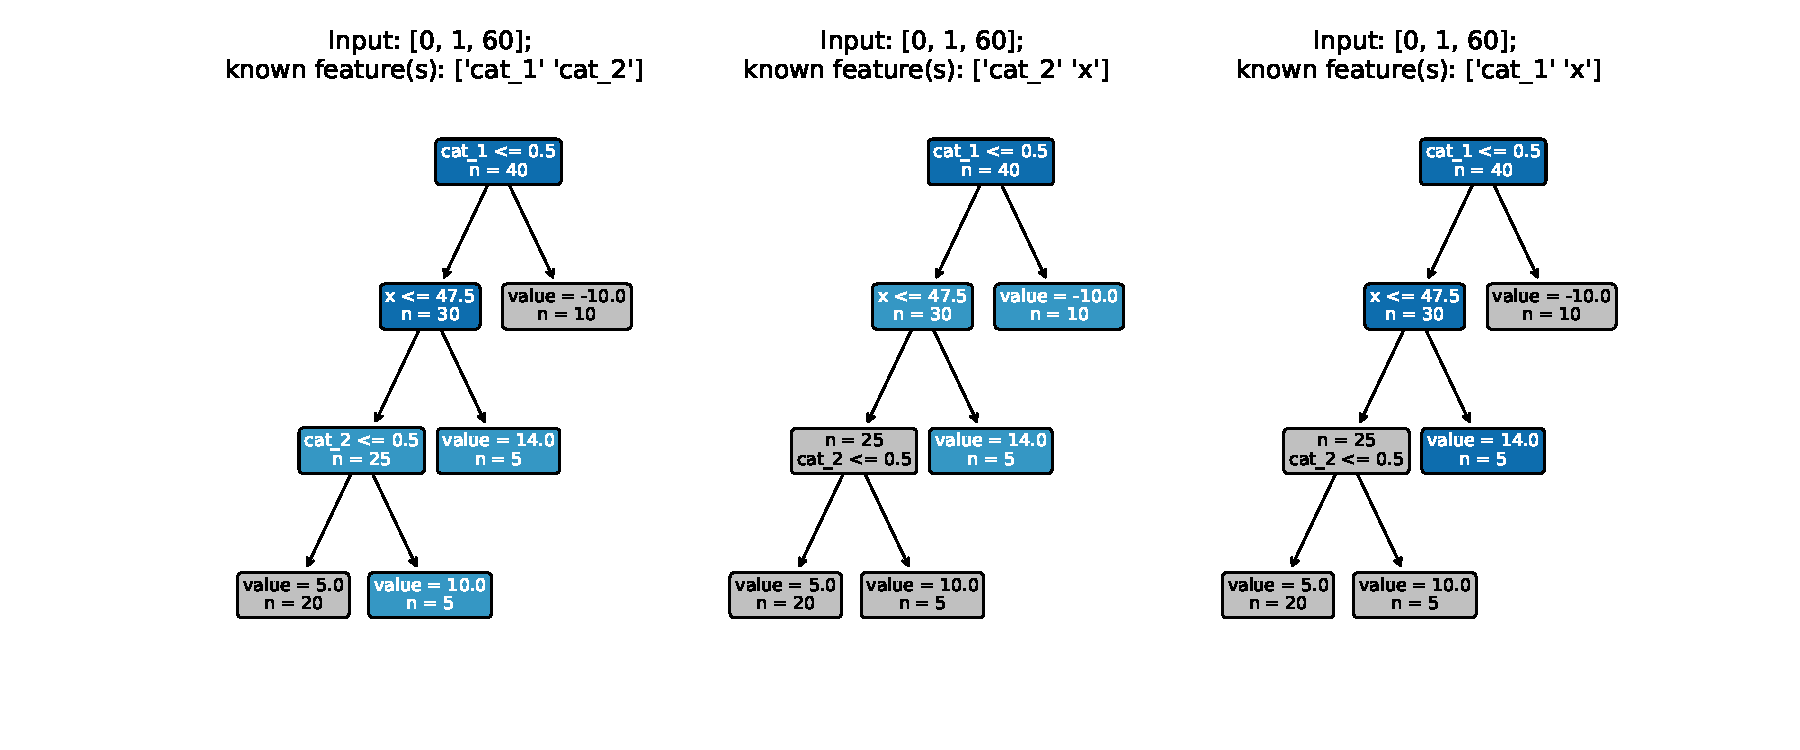
\includegraphics[height=6.6cm]{"../outputs/plot_tree/figures/path_2_known.pdf"}
    \caption{Plot of the fitted tree. The colored nodes correspond to the paths taken 
    by the algorithm when certain features of an input are known. Here, we consider that 
    two features are known.}
    \label{fig:tree2}
\end{figure}


Finally, we plot in figure (\ref{fig:tree3}) the tree paths when all the features are known: 
$$S = \{\text{cat}_1, \text{cat}_2, x\}.$$
We find that 
$$f_u(\{\text{cat}_1, \text{cat}_2, x\}) = 14$$

\begin{figure}[H]
    \centering
    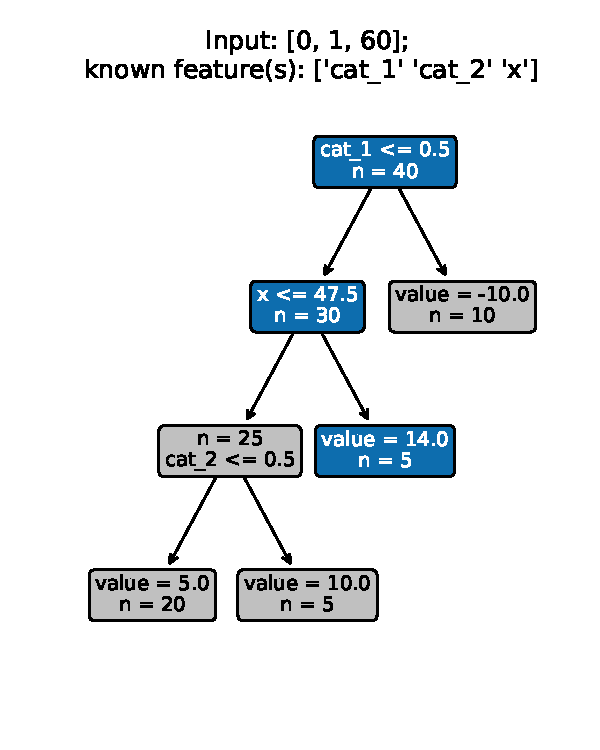
\includegraphics[height=9cm]{"../outputs/plot_tree/figures/path_3_known.pdf"}
    \caption{Plot of the fitted tree. The colored nodes correspond to the paths taken 
    by the algorithm when certain features of an input are known. Here, we consider that 
    three features are known.}
    \label{fig:tree3}
\end{figure}

By applying formula \ref{eq:shap} to each of the features, we obtain:
\begin{align*}
    & \phi_x = \frac{155}{36} \approx 4.3056\\
    & \phi_{\text{cat}_1} = \frac{191}{36} \approx 5.3056 \\
    & \phi_{\text{cat}_2} = \frac{25}{18} \approx 1.3889
\end{align*}

And on the other hand, if we redo the calculation considering that $\text{cat}_1$ and $\text{cat}_2$ form 
a set cat of cardinality 1 and are inseparable, the SHAP values become:
\begin{align*}
    & \phi_x' = \frac{25}{6} \approx 4.1667\\
    & \phi_{\text{cat}} = \frac{41}{6} \approx 6.8334
\end{align*}

We observe that $\phi_{\text{cat}} \neq  \phi_{\text{cat}_1}+\phi_{\text{cat}_2} $ and 
$\phi_x \neq  \phi_x'$. However, the values are quite close. Next, we will 
compare these two methods for different datasets to see if they lead to similar results.

\section*{Comparison of the two methods with generated datasets}

In order to compare the two methods, we modify the algorithm 2 Tree SHAP on page 4 of \cite{lundberg2019consistent}. 
This is a recursive algorithm that performs the calculations we have previously 
shown, in an optimal way without repeating values already calculated. In particular, we modify in the 
\texttt{RECURSE} procedure, the \texttt{FINDFIRST} function, which becomes a function searching for the first 
occurrence of any member of the feature group of the considered feature. We were inspired by the code in 
\href{https://github.com/shap/shap/blob/master/shap/explainers/_tree.py}{\_tree.py} to code our own version.

We also need to generate new datasets with categorical variables. Since all the algorithms are coded in \textit{Python}, 
the computation times are much longer than the original \textit{C++} algorithm. Therefore, we need to limit the size of 
the datasets and the number of trees in our predictive models.

To generate datasets, we use the functions \texttt{make\_classification} or \texttt{make\_regression} from
\texttt{sklearn.datasets}. These functions only provide numerical features. Therefore, we need to artificially 
transform numerical features into categorical variables by associating each value with a category based on its 
quantile. A random component is added to introduce errors in the category assignment.

In total, 120 datasets are generated (60 for binary classification and 60 for regression). They consist of 7 
features with 5 informative features. Among the datasets, we construct 1, 3, or 5 categorical variables in a 
balanced manner. All categorical variables contain 4 categories. The models used are random forest models with 
20 decision trees. The train/test ratio is 0.2.

The performance of the classification models are all acceptable, as reported in table \ref{table:perfo}. On the other hand, 
the regression models underperform. Therefore, we decide not to study the SHAP values of these models because 
it is not relevant to explain predictions of a model that does not perform well.

\begin{table}[H]
    \centering
    \begin{tabular}{cccc}
      \midrule
      & 1 categorical feature & 3 categorical features & 5 categorical features \\
      Accuracy & 0.82 & 0.81 & 0.75 \\
      Precision & 0.86 & 0.84 & 0.80 \\
      Recall & 0.81 & 0.79 & 0.71 \\
      \bottomrule
    \end{tabular}
    \caption{Average performance of the classification models for datasets containing 
    1, 3, 5 categorical features.}
    \label{table:perfo}
  \end{table}

Since transforming into categories causes a loss of precision in numerical variables, 
it is normal for performance to decrease as the number of categorical variables increases 
for the same total number of features.

For each of the datasets, we normalise the absolute values of the SHAP values so that the 
absolute values of the SHAP values for each prediction sum up to 1.

Then, we construct boxplots in figure \ref{fig:boxplot} to show the distribution of the mean differences of the 
normalized SHAP values calculated by the two methods for each prediction. We observe that the mean differences 
are very small for the most part. Indeed, in the most extreme cases, they barely exceed 3\%. This shows that 
the two methods seem to produce similar results.

\begin{figure}[H]
    \centering
    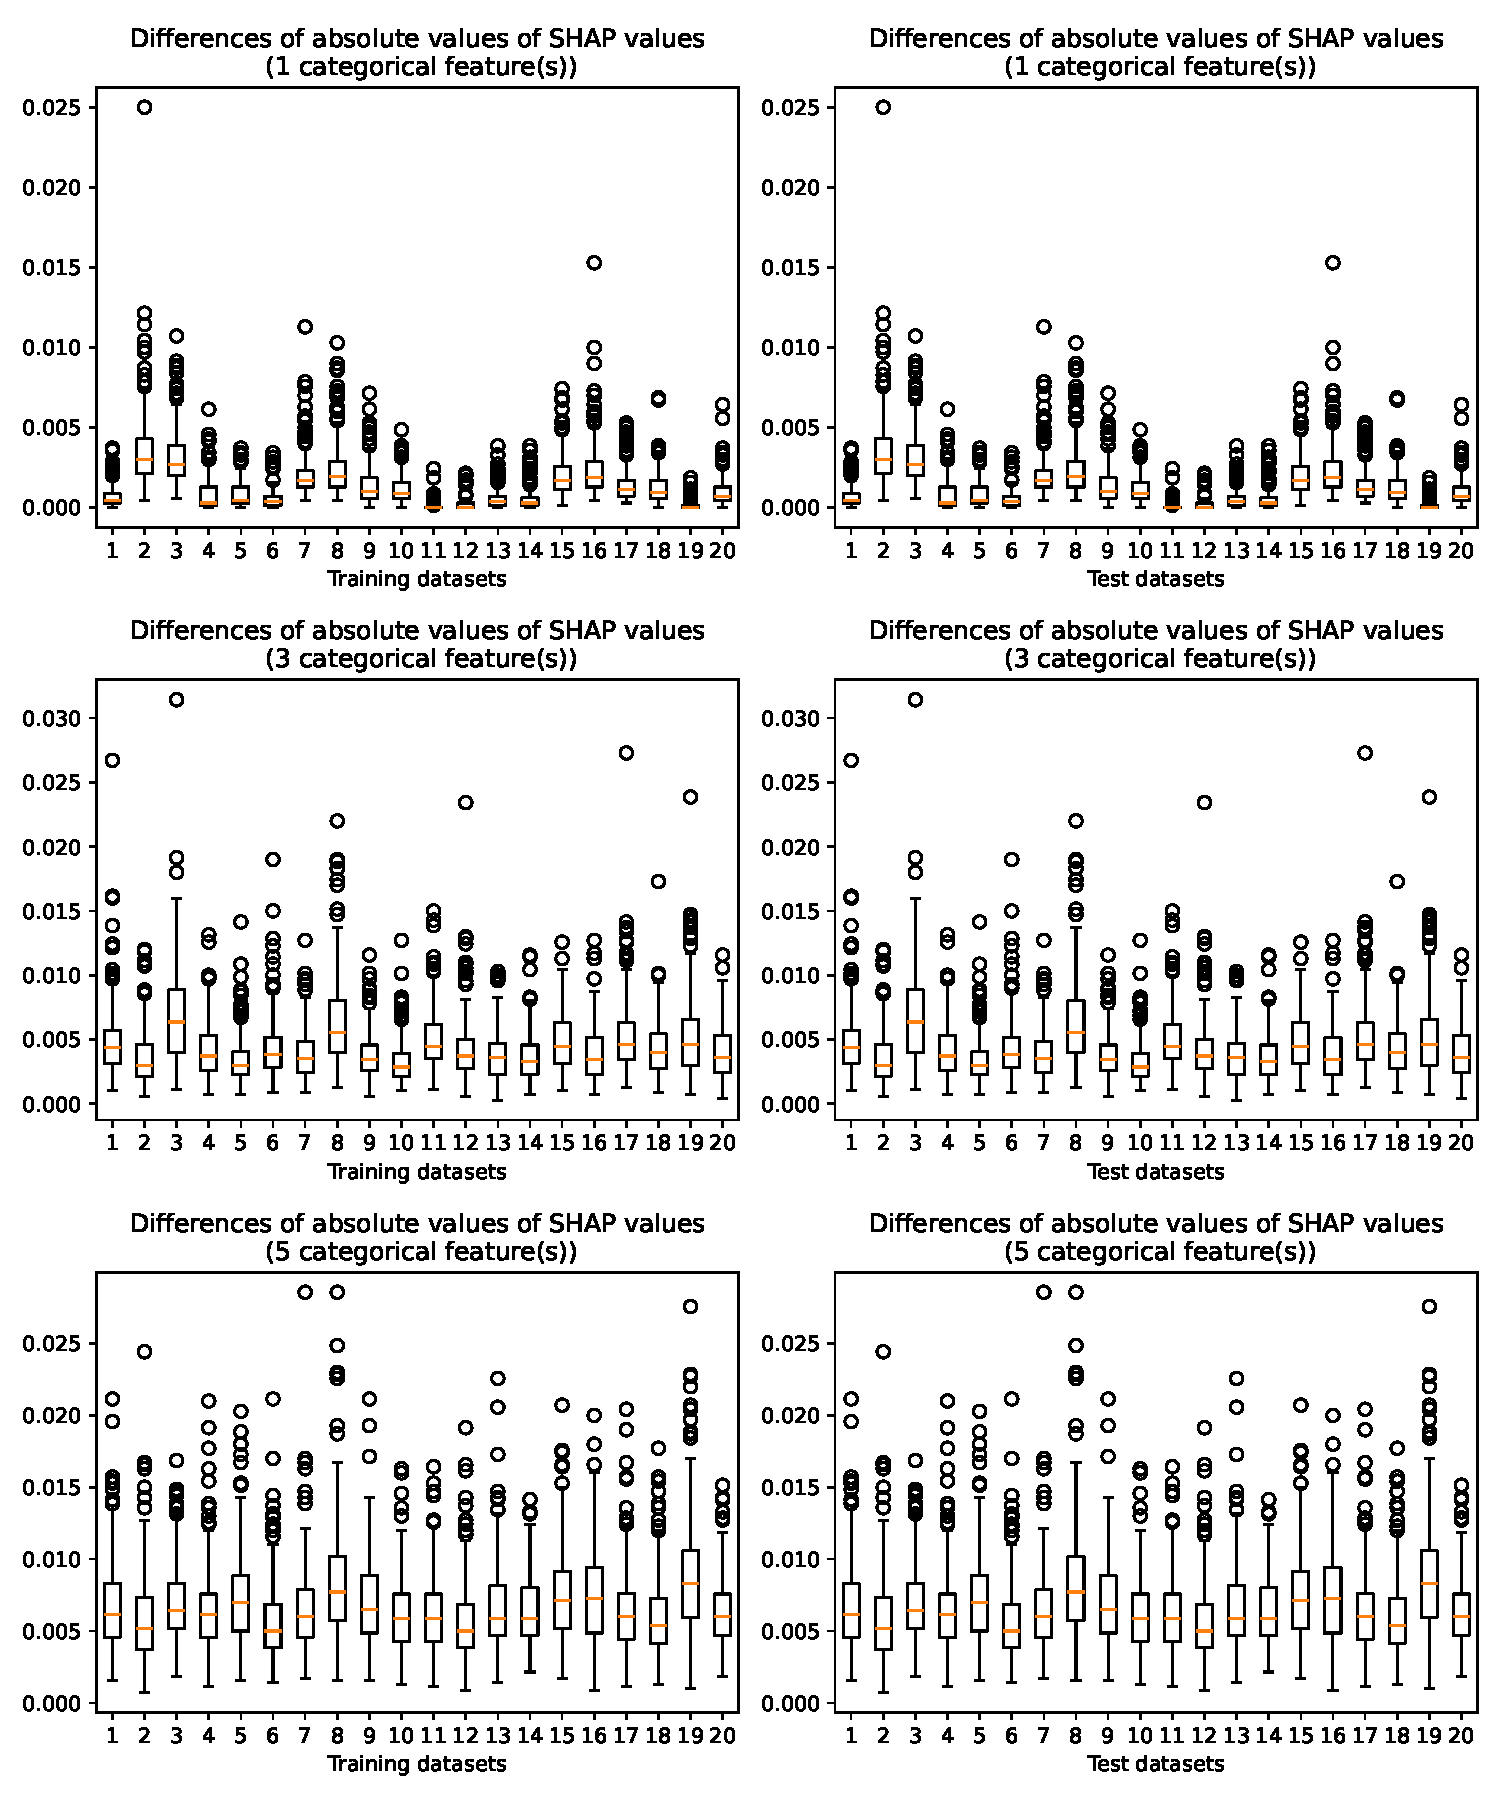
\includegraphics[height=15cm]{"../outputs/comparison-shap/figures/boxplots.pdf"}
    \caption{Boxplots of the absolute difference average of the absolute normalised SHAP values of both methods over
    the features for each prediction on the training and test set}
    \label{fig:boxplot}
\end{figure}

The SHAP values are also used to perform rankings from the most significant variable to the least significant one. 
It is therefore relevant to count, across the entire prediction set, the number of times the rankings differ.
More precisely, for each dataset configuration, we rank the absolute values of the normalized SHAP values 
that are greater than 10\%. We set this threshold to eliminate variables deemed insignificant that may 
disturb the end of the ranking. Then, we calculate the number of times the rankings differ and divide by the 
total number of predictions for the training and test sets.
We report the error rates in table (\ref{table:rankings}). We observe that as the number of categorical 
features increases, the rankings differ more. In the case of a dataset with many categorical variables, 
the differences become significant.

\begin{table}[H]
    \centering
    \begin{tabular}{cccc}
      \midrule
      & 1 categorical feature & 3 categorical features & 5 categorical features \\
      Training set & 0.05 & 0.15 & 0.25 \\
      Test set & 0.05 & 0.17 & 0.25 \\
      \bottomrule
    \end{tabular}
    \caption{Number of times the rankings differ divided by the total number of
     predictions for the training and test sets and given the number of categorical data.}
    \label{table:rankings}
  \end{table}


\newpage
\bibliography{bibliography}
\end{document}